\subsubsection{MF2. Modulo de generación y medición de la acústica}

Para este módulo, se hizo uso del entorno de MATLAB. El programa consiste en un dispositivo de reproducción y grabación simultanea, que envían una señal de excitación hacia el cuarto por medio de un altavoz, mientras un micrófono recoge tanto el sonido del altavoz como las reflexiones de las superficies del recinto. Posteriormente, el programa se encarga de utilizar la señal de excitación y la capturada, para estimar la respuesta al impulso del estudio.\hfill \break
Dentro del \textit{Audio Toolbox} de MATLAB (\href{https://www.mathworks.com/products/audio.html}{Liga al \textit{Toolbox}}) existe  el objeto \textit{AudioPlayerRecorder}, que nos permite escribir y leer paquetes de audio al dispositivo de la computadora. \hfill \break
Las primeras lineas del código están referidas a la inicialización y configuración del dispositivo de lectura y escritura.\hfill \break
\begin{lstlisting}[frame=single,numbers=left, style=Matlab-editor, basicstyle=\tiny]
clc; clear; close all;

fs = 44100;
room_dim = [6, 5, 3.5];
device = "ASIO4ALL v2";
aPR = audioPlayerRecorder("SampleRate",fs,"Device",device);
\end{lstlisting}
El dispositivo ``ASIO4ALL v2" \href{https://asio4all.org/}{(Liga a la pagina)} es un \textit{driver} para Windows, que nos permite utilizar los dispositivos de audio conectados a la computadora como tarjetas ASIO (\textit{Audio Stream Input-Output}) con la posibilidad de combinar dispositivos de entrada y salida. \hfill\break
Existen distintos métodos para medir la respuesta al impulso de un recinto, sin embargo, por la poca calibración que necesita para obtener resultados óptimos, además de que permite obtener un excelente ratio entre señal y sonido, el mejor método es el barrido senoidal. \href{https://people.montefiore.uliege.be/stan/ArticleJAES.pdf}{cita} \hfill\break
El barrido senoidal consiste en una señal senoidal, que aumenta de frecuencia conforme avanza el tiempo. El dispositivo ASIO emite la señal mientras va leyendo la respuesta del recinto. Se puede estimar la respuesta al impulso al realizar una deconvolucion entre la señal emitida y la capturada. El siguiente paso en el código es definir los parámetros del barrido senoidal, como la amplitud, rango y duración.
\begin{lstlisting}[frame=single,numbers=left, style=Matlab-editor, basicstyle=\tiny]
sweep_dur = 5;
duration_per_run = 8;
start_silence = 1;
silence_dur = duration_per_run - sweep_dur - start_silence;
sweep_range = [10 8000];
percentage = 100;
outputLevel = 20*log10(percentage/100);
sweepsine = sweeptone(sweep_dur,silence_dur,fs,"SweepFrequencyRange", ...
    sweep_range,"ExcitationLevel",outputLevel);
\end{lstlisting}
Para asegurar la simultaneidad de las señales de entrada es salida, es necesario utilizar \textit{buffers} que se encargaran de gestionar el flujo de datos. Además, se incluyen tiempos de silencio al antes y después de la señal, que permita compensar por pequeños desfases.
\begin{lstlisting}[frame=single,numbers=left, style=Matlab-editor, basicstyle=\tiny]
excitation = [zeros(start_silence*fs,1); sweepsine];
sampling = 1024;
excitation_length = length(excitation);
bufOut = dsp.AsyncBuffer(excitation_length);
bufIn = dsp.AsyncBuffer(excitation_length);
write(bufOut,excitation);
\end{lstlisting}
Se leerán y escribirán datos a la tarjeta de audio mediante paquetes de 1024 muestras, hasta que se acaben los datos del \textit{buffer}.
\begin{lstlisting}[frame=single,numbers=left, style=Matlab-editor, basicstyle=\tiny]
while bufOut.NumUnreadSamples > 0
    exci = read(bufOut,sampling);
    [rec,num_under,num_over] = aPR(exci);
    write(bufIn,rec);
    if num_under>0 || num_over>0
        fprintf("Underrun by %d frames, overrun by %d frames.\n",num_under,num_over)
    end
end
release(aPR);
read(bufIn,start_silence*fs);
audioFromDevice = read(bufIn);
\end{lstlisting}

Por ultimo, se hace el proceso de deconvolucion mediante la funcion de matlab \textit{impzest}, se normaliza para tener amplitud de 1 y se crea el vector de tiempo. Los datos de la respuesta al impulse se guardan en una estructura junto con el tiempo de muestreo $f_{s}$.

\begin{lstlisting}[frame=single,numbers=left, style=Matlab-editor, basicstyle=\tiny]
time = (1:length(audioFromDevice))/fs;
RIR = impzest(sweepsine,audioFromDevice);
[max_RIR,Idx] = max(abs(RIR));
n_RIR = RIR(Idx-round(fs/100):end)/max_RIR;
time_RIR = (1:length(n_RIR))/fs;
ImpulseResponse.fs = fs;
ImpulseResponse.y = n_RIR;

plot(time,audioFromDevice)
title('Audio recorded')
xlabel('Time(s)')
ylabel('Amplitude')

plot(time_RIR, n_RIR)
title('Estimated impulse response')
xlabel('Time(s)')
ylabel('Amplitude')
\end{lstlisting}

Las gráficas resultantes, muestran la señal de excitación, la grabación y la estimación de la respuesta al impulso.
\begin{figure}[!htb]
    \centering
     \begin{subfigure}{0.3\textwidth}
        \centering
        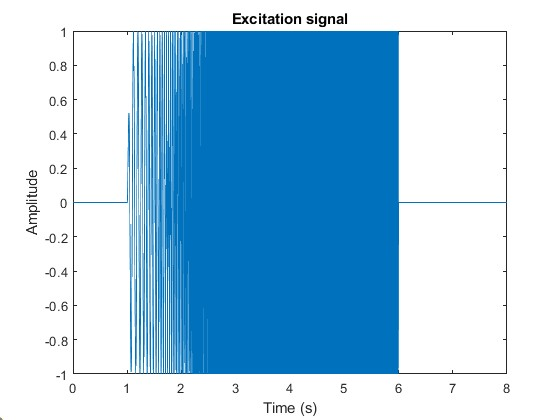
\includegraphics[width=\linewidth]{imagenes/ExcitationSignal_RIR_Measurement.jpg}
        \caption{\footnotesize Señal de excitación (Barrido senoidal)}
        \label{fig:sub1}
    \end{subfigure}
    \hfill
    \begin{subfigure}{0.3\textwidth}
        \centering
        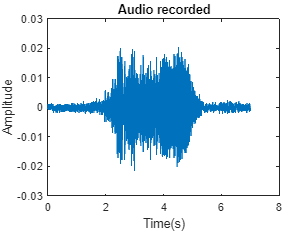
\includegraphics[width=\linewidth]{imagenes/AudioFromDevice_RIR_Measurement.png}
        \caption{\footnotesize Audio grabado}
        \label{fig:sub2}
    \end{subfigure}
    \hfill
    \begin{subfigure}{0.3\textwidth}
        \centering
        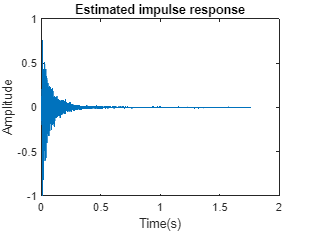
\includegraphics[width=\linewidth]{imagenes/EstimatedImpulseResponse_RIR_Measurement.png}
        \caption{\footnotesize Respuesta al impulso estimada}
        \label{fig:sub2}
    \end{subfigure}
    \caption{Gráficas resultantes de generación y medición de la acústica}
\end{figure}
\FloatBarrier

El programa completo se encuentra como () en el Anexo ().
%------------------------------------------------------------------------
